% --------------------------------------------------------------
% This is all preamble stuff that you don't have to worry about.
% Head down to where it says "Start here"
% --------------------------------------------------------------

\documentclass[10pt]{beamer}

% \usepackage[margin=1in]{geometry}
\usepackage{amsmath,amsthm,amssymb,mathrsfs}
\usepackage{tikz}
\usepackage{wrapfig}
\usepackage{cjhebrew}
% \usepackage[shortlabels]{enumerate}

\usepackage[utf8]{inputenc}
\usepackage[english]{babel}

\usetikzlibrary{calc}
\usetikzlibrary{arrows.meta}
\usetikzlibrary{arrows}

\title[$p$-Laplacian and max flow/min cut]{The $p$-Laplacian, laminations, and max flow/min cut}
\author{Aidan Backus}

\newcommand{\NN}{\mathbb{N}}
\newcommand{\ZZ}{\mathbb{Z}}
\newcommand{\QQ}{\mathbb{Q}}
\newcommand{\RR}{\mathbb{R}}
\newcommand{\CC}{\mathbb{C}}


\newcommand*\dif{\mathop{}\!\mathrm{d}}
\DeclareMathOperator*{\argmin}{argmin}
\DeclareMathOperator{\dist}{dist}
\DeclareMathOperator{\supp}{supp}
\DeclareMathOperator{\Var}{Var}
\DeclareMathOperator{\Exc}{Exc}
\DeclareMathOperator*{\Expect}{\mathbf E}
\newcommand{\normal}{\vec n}
\newcommand{\norm}[1]{\left\lVert#1\right\rVert}

\newcommand{\Spec}{\operatorname{Spec}}

\renewcommand{\Re}{\operatorname{Re}}
\renewcommand{\Im}{\operatorname{Im}}

\newtheorem{theoremconjecture}{Theorem-Conjecture}
\newtheorem{conjecture}{Conjecture}
\newtheorem{proposition}{Proposition}
\newtheorem{question}{Question}

\usepackage[backend=bibtex,style=alphabetic,maxcitenames=50,maxnames=50]{biblatex}
\addbibresource{ultrapowerful.bib}
\renewbibmacro{in:}{}
\DeclareFieldFormat{pages}{#1}

\usetheme{AnnArbor}
\usecolortheme{dove}

\begin{document}
% --------------------------------------------------------------
%                         Start here
% --------------------------------------------------------------
\begin{frame}
    \titlepage
\end{frame}

\begin{frame}{Max flow min cut}
\begin{itemize}
\item The \emph{max flow min cut theorem} asserts that in a discrete flow network, the maximal amount of incompressible fluid that can flow equals the capacity of the smallest bottleneck. \pause
\item Picture from Wikipedia:
\end{itemize}

\begin{center}
    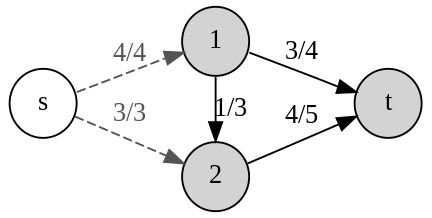
\includegraphics[scale=0.75]{Max-flow_min-cut_example.svg.png}
\end{center}
\end{frame}

\begin{frame}{A continuous max flow min cut?}
\begin{itemize}
\item Various formulations of a continuous max flow/min cut theorem (for example Sullivan '90, Thurston '96, Grieser '05, Freedman and Headrick '16). \pause
\item MF/MC arises from the convex duality theorem applied to the space of $\ell^\infty$ functions on the space of edges. \pause
\item So, natural to prove a continuous MF/MC theorem that arises from convex duality on $L^\infty$. \pause
\item $L^\infty$ is not reflexive, so we will regularize by using $L^q$, $q < \infty$.
\end{itemize}
    
\end{frame}

\begin{frame}{\texorpdfstring{The $p$-Laplacian}{The p-Laplacian}}
\begin{itemize}
\item We will look at the (regularized) dual problem first. It is the $p$-Laplacian: to minimize
$$J_p(u) := \frac{1}{p} \int_M |\nabla u(x)|^p \dif x,$$
the $p$-Dirichlet energy, where we always have $1/p + 1/q = 1$. \pause
\item Its convex dual is the minimization of
$$\hat J_p(F) = -\frac{1}{q} \int_M |F(x)|^q \dif x$$
where $F$ ranges over $d - 1$-forms subject to the constraint $\dif F = 0$. \pause
\item Taking $p \to 1$ we get
$$J_1(u) := \int_M |\nabla u(x)| \dif x = \sup_{\substack{\varphi \in C^1_0(M, \Omega^{d - 1}) \\ \|\varphi\|_{C^0} \leq 1}} \int_M u \dif \varphi$$
which is the least gradient energy in the weak sense.
\end{itemize}
\end{frame}

\begin{frame}{Functions of least gradient}
\begin{itemize}
\item We say that $u \in BV(M)$ has \emph{least gradient} if $u$ minimizes $J_1$ subject to Dirichlet (or equivariant) boundary conditions. \pause
\item Let $\mathcal H^s$ denote $s$-dimensional Hausdorff measure. Then
$$J_1(u) = \int_{-\infty}^\infty \mathcal H^{d - 1}(\partial \{u > t\}) \dif t$$
for any $u \in BV(M)$. \pause
\item Thus the level sets of a least gradient function $u$ are area-minimizing. They are also all disjoint (Auer and Bangert '02). \pause
\end{itemize}

\begin{theorem}[Bombieri, de Giorgi, Giusti '69]
Suppose that $u \in BV(M)$ has least gradient.
Then for every $t \in \RR$ and every hypersurface $\Sigma$ homologous to $\partial \{u > t\}$ relative to $\partial M$,
$$\mathcal H^{d - 1}(\partial \{u > t\}) \leq \mathcal H^{d - 1}(\Sigma).$$
In particular, $\Sigma$ is a smooth complete hypersurface.
\end{theorem} 
\end{frame}

\begin{frame}{Laminations}
\begin{itemize}
\item A \emph{lamination} $\lambda$ in $M$ is a partition of a closed set $S$ into complete hypersurfaces, called \emph{leaves}, such that we can cover $M$ by small balls $B$, called \emph{flow boxes} such that $S \cap B \cong K \times \RR^{d - 1}$ for some compact set $K \subset \RR$, where $\{k\} \times \RR^{d - 1}$, $k \in K$, is $\Sigma \cap B$ for a leaf $\Sigma$. \pause
\item We say that $\lambda$ is \emph{Lipschitz}, if the change-of-coordinates maps between flow boxes can be chosen to be Lipschitz. \pause
\item Picture by Thurston '79:
\end{itemize}

\begin{center}
    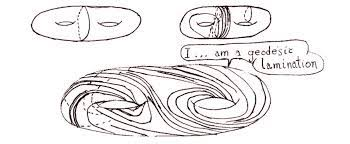
\includegraphics[scale=0.68]{GeodesicLamination.jpg}
\end{center}
\end{frame}

\begin{frame}{Ruelle-Sullivan currents}
\begin{itemize}
\item Let $\lambda$ be a lamination. A \emph{Ruelle-Sullivan current} $T$ for $\lambda$ is a continuous linear function on $C^0_0$ $d - 1$-forms $\varphi$, such that if $\varphi$ is supported in a flow box $B$ with $S \cap B \cong K \times \RR^{d - 1}$,
$$\langle T, \varphi\rangle = \int_K \int_{\{k\} \times \RR^{d - 1}} \varphi \dif \mu(k)$$
for some Radon measure $\mu$ with support $K$. \pause
\item A \emph{measured oriented lamination} is the data of a lamination and a Ruelle-Sullivan current. \pause
\item Daskalopolous and Uhlenbeck '20 observed that a for wide class of functions of least gradient $u$ on the hyperbolic plane, $\dif u$ is the Ruelle-Sullivan current of a geodesic lamination and conjectured that this was true more generally.
\end{itemize}
\end{frame}

\begin{frame}{Least gradient functions and Ruelle-Sullivan currents}
\begin{theorem}[B '23]
Suppose that $u$ is a function of least gradient. Then there exists a Lipschitz lamination $\lambda$ whose leaves are the level sets $\partial \{u > t\}$ of $u$.
Moreover, $\dif u$ is a Ruelle-Sullivan current of $\lambda$.
\end{theorem} \pause

\begin{itemize}
    \item Proof is based on elliptic estimates for area-minimizing hypersurfaces, especially Harnack's inequality. \pause
    \item A partial converse is also available; together these results completely characterize function of least gradient. \pause
    \item So after a Lipschitz change of coordinates, $u$ is constant in $d - 1$ directions. This gives a new proof of the following regularity theorem for least gradient functions: \pause
\end{itemize}

\begin{theorem}[Hakkarainen et al '15, G\'orny '18]
Suppose that $u$ is a function of least gradient. 
Then $u = u_{ac} + u_C + u_j$ where $u_{ac}, u_C, u_j$ have least gradient, $u_{ac} \in W^{1, 1} \cap C^0$, $u_C \in C^0$ is a Cantor function, and $u_j$ is a jump function.
\end{theorem}
\end{frame}

% \begin{frame}{The lamination construction theorem}
% \begin{itemize}
% \item One can use curvature estimates for area-minimizing hypersurfaces (Schoen and Simon '81) to reduce the least gradient-lamination correspondence theorem to: \pause
% \end{itemize}

% \begin{theorem}[B '23, following Solomon '86]
% Let $\mathscr S$ be a set of disjoint minimal hypersurfaces whose second fundamental forms are locally uniformly bounded.
% Then $\mathscr S$ is the set of leaves of a Lipschitz lamination.
% \end{theorem} \pause

% \begin{itemize}
% \item Main idea: by disjointness, on small scales the hypersurfaces must all be graphs over each other, of functions which are small-data solutions of the minimal surface equation. Then use Harnack-type estimates. \pause
% \item One can use this theorem to show compactness theorems for certain spaces of laminations as well.
% \end{itemize}
% \end{frame}

\begin{frame}{Continuous max flow min cut}
\begin{itemize}
\item Thurston '96 conjectured that a MF/MC theorem should be available for laminations but wasn't precise about what he meant. \pause
\item Recall that the convex dual problem to the $q$-Laplacian is the minimization of
$$\hat J_q(F) = \frac{1}{p} \int_M |F(x)|^p \dif x$$
where $F$ ranges over $d - 1$-forms such that $\dif F = 0$. \pause
\item The convex duality relation is 
$$\frac{1}{q} \int_M |\dif u|^q + \frac{1}{q} \int_M |F|^p + \int_M \dif u \wedge F.$$
\item We are going to construct an ``incompressible flow'' out of $F$ as $p \to \infty$ which is bottlenecked by a lamination obtained from the limit of $u$ as $q \to 1$.
\end{itemize}
\end{frame}

\begin{frame}{The dual forms}
\begin{itemize}
\item We say that a $d - 1$-form $F_p$ is \emph{$p$-tight} if $F_p$ minimizes $\hat J_p$ subject to $\dif F_p = 0$, among all $F_p$ cohomologous to $F$ relative to the boundary. \pause
\item If $u_q$ is $q$-harmonic, then
$$F_p := |\dif u_q|^{q - 2} \star \dif u_q$$
is $p$-tight.
\item $p$-tight forms essentially appear in the weak formulation of $1$-harmonic functions (Maz\'on, Rossi, and Segura de L\'eon '14), and in applications to Teichm\"uller theory (Daskalopolous and Uhlenbeck '20, '22) though neither paper made this explicit.
\end{itemize}
\end{frame}

\begin{frame}{The tight form}
\begin{itemize}
\item We say that $F$ is \emph{tight} if there are $p$-tight $F_p$ such that $F_p \to F$ weakly in $L^r$ for every $1 < r < \infty$. \pause
\item If $F$ is tight, then $F$ minimizes its $L^\infty$ norm among all $d - 1$-forms cohomologous to $F$ relative to the boundary. \pause
\item On the level of formal manipulations, $F$ is tight iff
\begin{equation}\label{tight PDE}
\begin{cases}
\dif F = 0 \\
(\nabla_i F_{j_1 \cdots j_{d - 1}}) F^{j_1 \cdots j_{d - 1}} {F^i}_{k_1 \cdots k_{d - 2}} = 0.
\end{cases}
\end{equation}
But (\ref{tight PDE}) makes no sense because viscosity solutions are ill-defined for systems and a tight form only satisfies $F \in L^\infty$. \pause 
\item In fact, for $d = 3$ there is a smooth solution of (\ref{tight PDE}) which is not tight and is not an $L^\infty$ minimizer.
\end{itemize}
\end{frame}

\begin{frame}{The duality theorem}
\begin{theorem}[B, in preparation]
Suppose that $M$ is closed oriented, $\rho \in H^{d - 1}_{\rm dR}(M, \RR)$, and $F_p$ the $p$-tight representatives of $\rho$.
Let $u_q$ be the $F_p$-conjugate $q$-harmonic equivariant functions on $\tilde M$ ($p^{-1} + q^{-1} = 1$).
Then $u_q \to u$ weakly in $BV$ and $F_p \to F$ weakly in $L^r$ ($1 < r < \infty$) as $q \to 1$, where $u$ has least gradient and $F$ is tight. 
Furthermore, 
\begin{equation}\label{duality equation}
\dif u \wedge F = \|F\|_{L^\infty} \star |\dif u|.
\end{equation}
\end{theorem} \pause

\begin{itemize}
\item The key point of the proof is that (\ref{duality equation}) is the convex duality relation for tight forms and least gradient functions. After proving this result, it necessarily follows that $u$ has least gradient (since $F$ is by definition tight). \pause
\item The total measure $\|\kappa\|$ of the measured oriented lamination $\kappa$ associated to $u$ is as small as possible, so we may view it as a ``minimal cut''. \pause
\item Conversely, $F$ is bottlenecked by $\kappa$ in the following sense:
\end{itemize}
\end{frame}

\begin{frame}{Continuous max flow min cut}
\begin{theorem}[B, in preparation]
Suppose that $M$ is closed oriented, and $F$ is a tight form which is dual to a least gradient function $u$ in the sense of (\ref{duality equation}).
Let $\kappa$ be the measured oriented lamination from $u$.
Then $\kappa$ is characterized as the measured oriented lamination which maximizes $\|\lambda\|^{-1} \int_\lambda F$.
\end{theorem} \pause

\begin{itemize}
\item Once we show that $\int_\lambda F$ is well-defined, this easily follows from (\ref{duality equation}). \pause
\item Think of $F$ as a divergence-free vector field. Following Freedman and Headrick '16, the continuous analogue of an incompressible flow is a divergence-free vector field of $L^\infty$ norm at most $1$. \pause
\item We can normalize $\|F\|_{L^\infty} = 1$, then the theorem says: \pause
\begin{itemize}
\item We must have $|F| = 1$ on every leaf $\Sigma$ of $\kappa$, and $F$ normal to $\Sigma$ (Bernoulli's principle). \pause
\item If $G$ is an incompressible flow cohomologous to $F$, then the same holds for $G$.
\end{itemize}
\end{itemize}
\end{frame}

\end{document}
